%%%% fatec-article.tex, 2024/03/10

\documentclass[
  a4paper,%% Tamanho de papel: a4paper, letterpaper (^), etc.
  12pt,%% Tamanho de fonte: 10pt (^), 11pt, 12pt, etc.
  english,%% Idioma secundário (penúltimo) (>)
  brazilian,%% Idioma primário (último) (>)
]{article}

%% Pacotes utilizados
\usepackage[]{fatec-article}

%% Início do documento
\begin{document}
\vspace{8cm}
\begin{center}
    \large \textbf{\title{ARTEFATOS DO PROJETO DE SOFTWARE}}
\end{center}

\maketitle

\break

\tableofcontents

\break


%exemplo da forma de organização das seções e subseções, você deverá adaptar o template para a realidade do seu projeto.

\section*{Diagramas UML}
    Nesta seção serão apresentados os diagramas da UML utilizados para a modelagem do sistema desenvolvido. Dentre os diagramas utilizados, pode-se citar: Diagrama de Caso de Uso, Modelo Lógico, Modelo Conceitual, Dicionário de dados e Diagrama de Redes
    
    \subsection*{Diagrama de Caso de Uso}
    \addcontentsline{toc}{section}{Diagrama de Caso de Uso}

    O diagrama a seguir foi desenvolvido para o aplicativo CitrosGuard, ele tem como funcionalidade demonstrar como é o uso do aplicativo e como o usuario, o sistema e os administradores tem como função no aplicativo, o diagrama conta com todas as funcionalidades do sistema.

            \begin{figure}[h]
\centering
\caption{Diagrama de caso de uso}%
\label{fig:diagrama-caso-uso}
 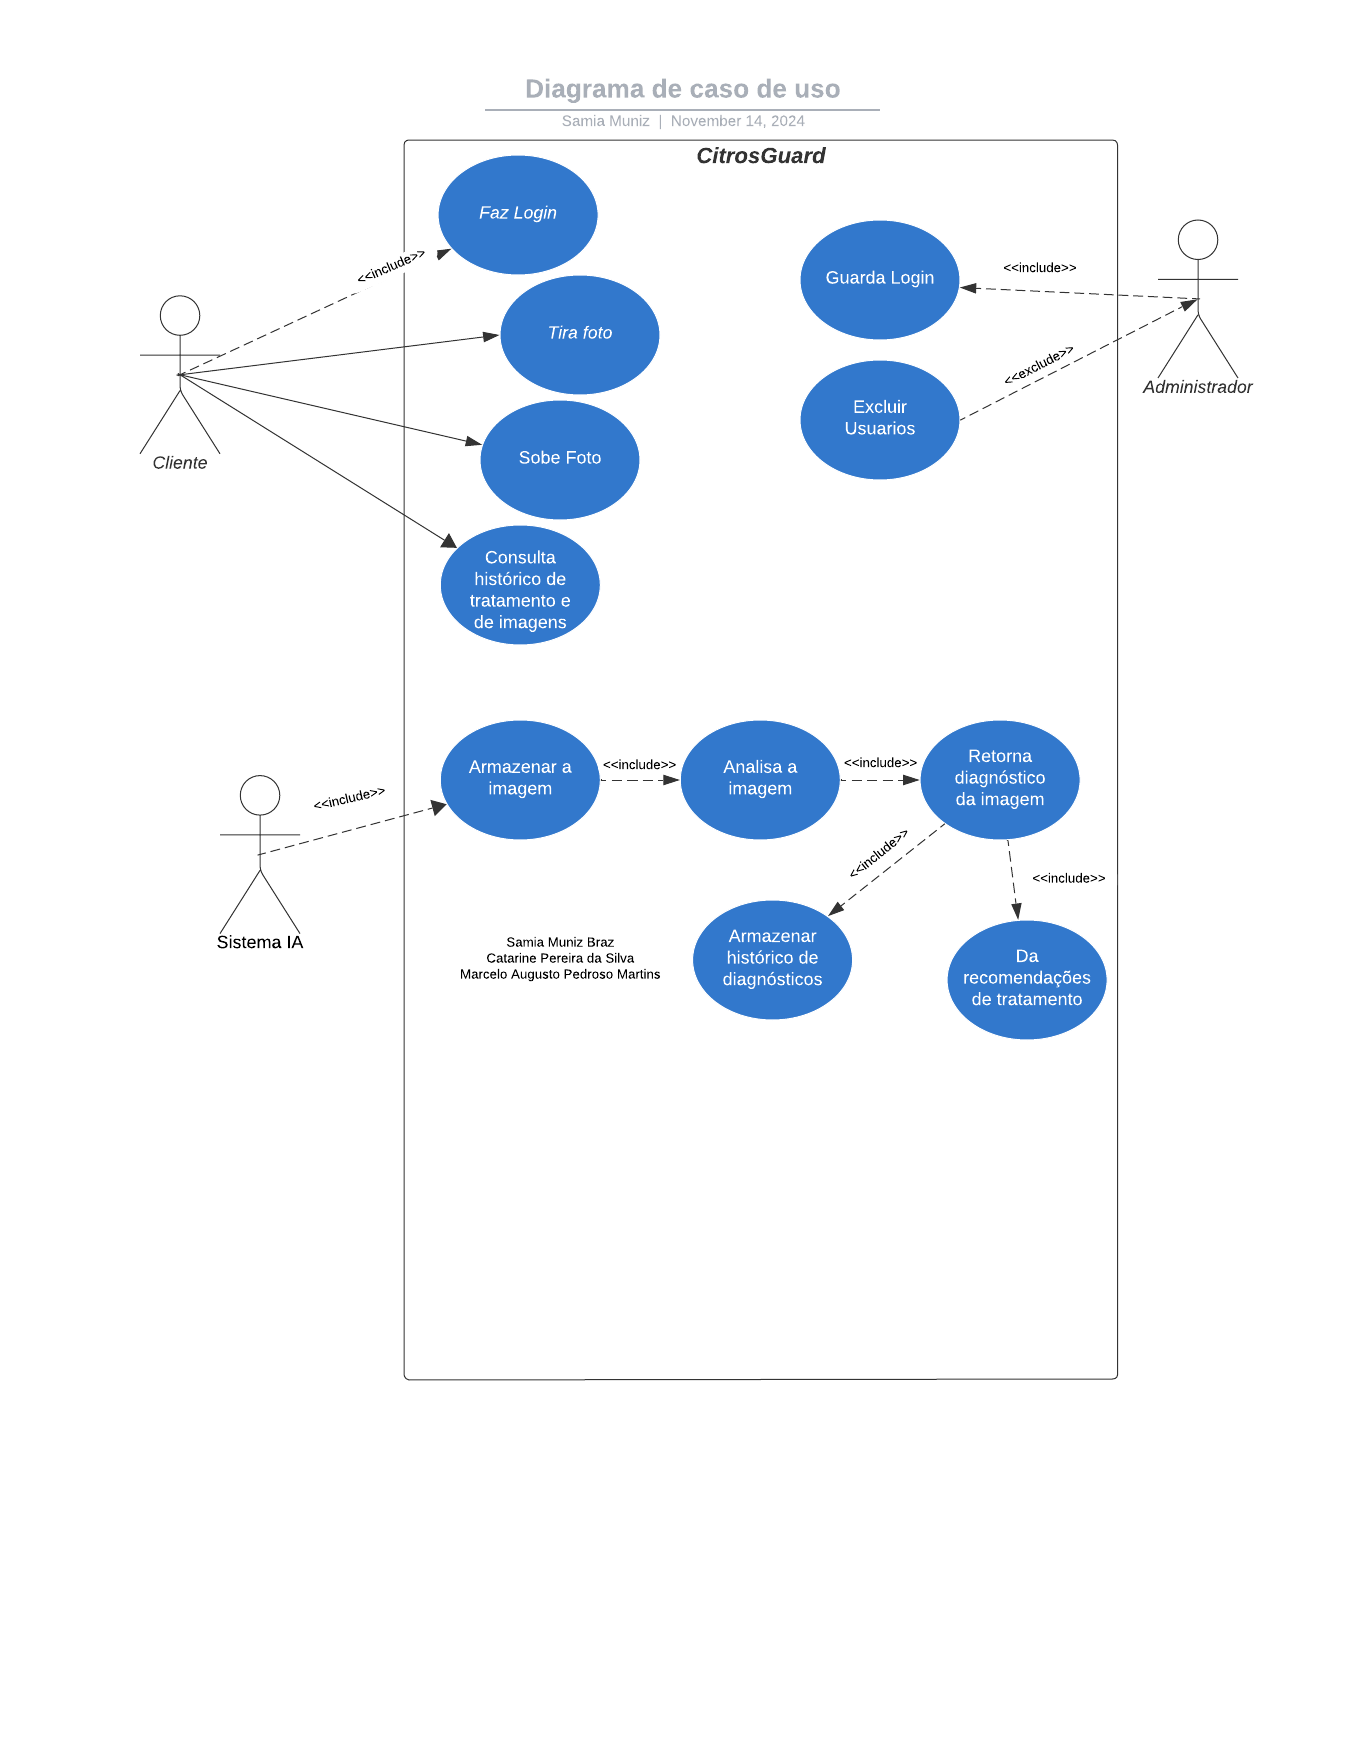
\includegraphics[width=0.75\textwidth]{Logos/Diagrama de caso de uso.png}
\SourceOrNote{Lucidchart (2024)}
\end{figure}

    Diagrama de caso de uso do aplicativo em desenvolvimento CitrosGuard
    
    \subsection*{Modelo Conceitual}
    \addcontentsline{toc}{section}{Modelo conceitual}

    O Modelo Conceitual a seguir foi desenvolvido para o banco de dados do aplicativo CitrosGuard e para o banco de dados do Apex, ele demonstra todos os relacionamentos que o usuário terá em tirar a foto do tronco ou fruto que acha que está contaminado até a imagem chegar ao nosso banco de dados.

    \begin{figure}[h]
\centering
\caption{Modelo Conceitual}%
\label{fig:diagrama-conceitual}
 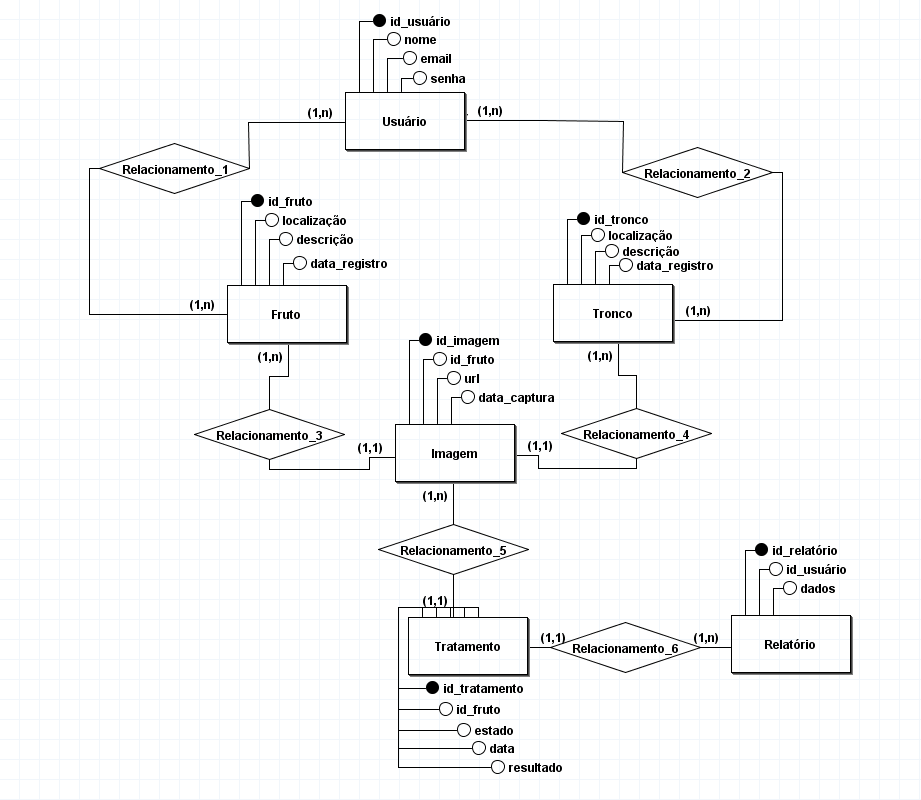
\includegraphics[width=0.8\textwidth]{Logos/diagrama de classe.png}
\SourceOrNote{BrModelo (2024)}
\end{figure}

     O diagrama foi desenvolvido no aplicativo BrModelo e explica como o usuário vai interagir com as funcionalidades que o sistema propõe

    \subsection*{Modelo Lógico}
    \addcontentsline{toc}{section}{Modelo Lógico}

    O banco de dados é de suma importância para o armazenamento de informações e a organização desses dados, a modelagem conceitual e lógica demonstram a funcionalidade do programa. No modelo lógico é possível observar a parte mais factual do projeto, demonstrando como o modelo real do banco de dados será construído O banco de dados é de suma importância para o armazenamento de informações e a organização desses dados, a modelagem conceitual e lógica demonstram a funcionalidade do programa. No modelo lógico é possível observar a parte mais factual do projeto, demonstrando como o modelo real do banco de dados será construído  

        \begin{figure}[h]
\centering
\caption{Diagrama de objetos}%
\label{fig:diagrama-logico}
 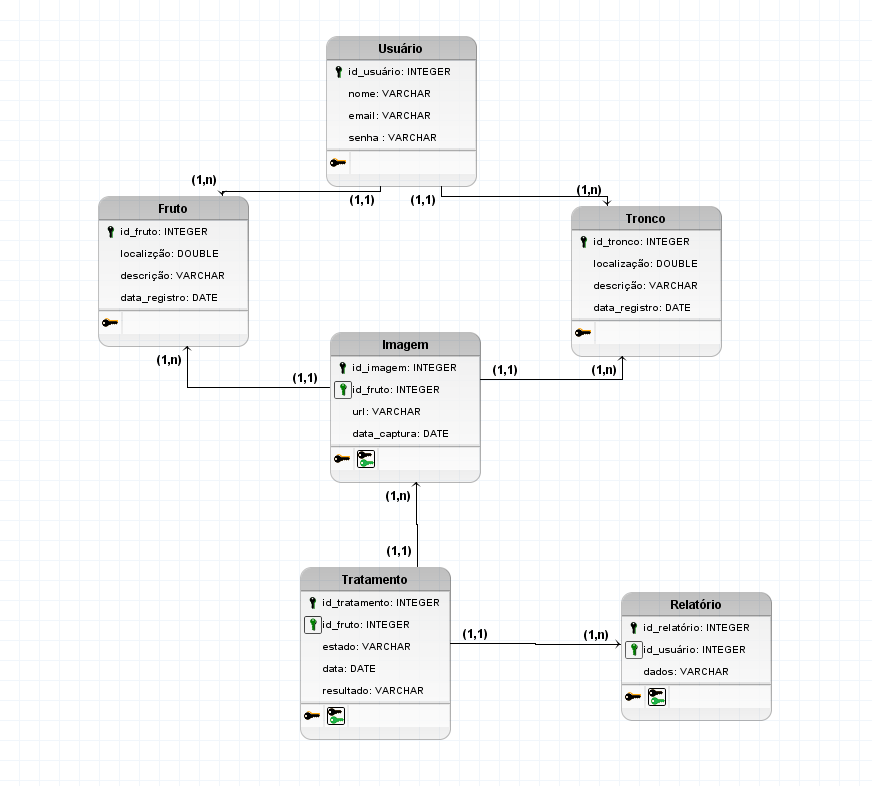
\includegraphics[width=0.9\textwidth]{Logos/logico.png}
\SourceOrNote{BrModelo (2024)}
\end{figure}

\subsection*{Diagrama de Rede}
    \addcontentsline{toc}{section}{Diagrama de Rede}

    Conforme o diagrama de redes a seguir é possível a visualização das redes e de como a comunicação do sistema vai funcionar. Na imagem é possível ver que a IA (inteligência artificial) irá se comunicar com o banco de dados do nosso sistema fazendo uploads constantes sobre os usuários e as fotos que eles possam subir pelo aplicativo. O banco de dados se comunicará com o computador dos administradores para possíveis mudanças e atualização e o banco também será responsável por gerar documentos e relatórios sobre o aplicativo. A figura abaixo do banco representa o usuário se comunicando com o aplicativo mobile e o aplicativo mobile fazendo upload de todas as informações que o usuário digitou e mandou pelo aplicativo.

    \begin{figure}[h]
        \centering
        \caption{Diagrama de Rede}%
        \label{fig:diagrama-rede}
         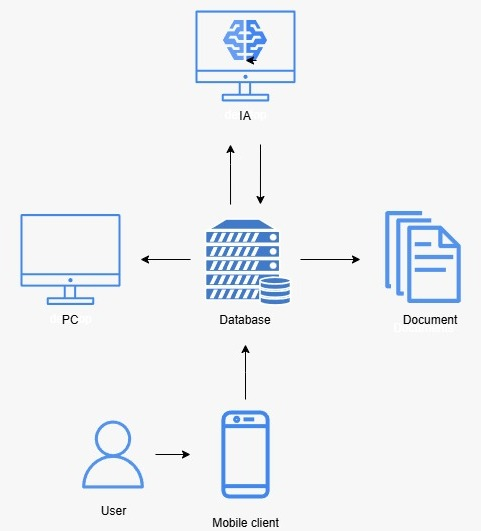
\includegraphics[width=0.9\textwidth]{Logos/diagrama de rede.jpg}
        \SourceOrNote{Lucidchart (2024)}
        \end{figure}

\subsection*{Canva}
\addcontentsline{toc}{section}{Canva}

O Canva a seguir mostra o público-alvo do projeto e ilustra como o aplicativo de identificação da gomose pode atender às necessidades de pequenos e médios produtores rurais, técnicos agrícolas e engenheiros agrônomos.

\begin{figure}[h]
    \centering
    \caption{Canva}%
    \label{fig:diagrama-canva}
     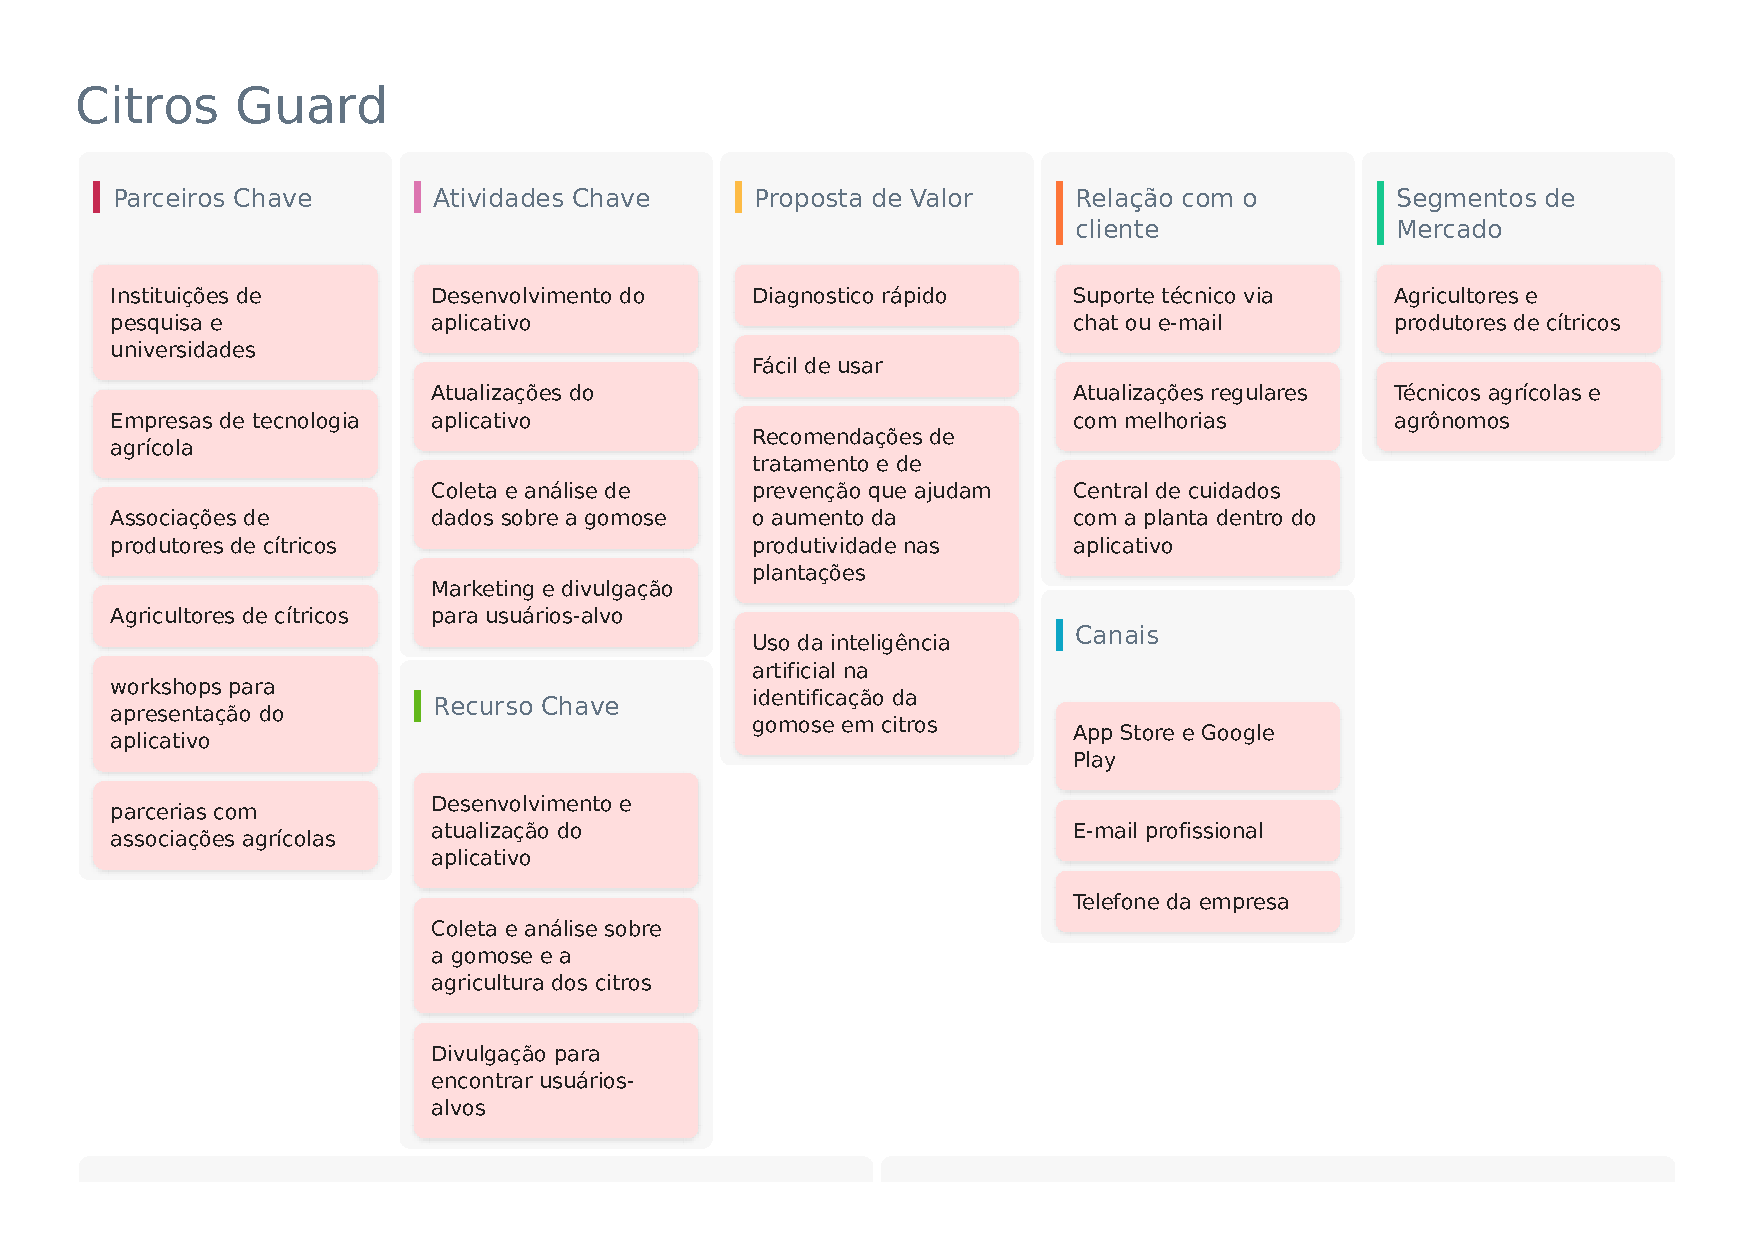
\includegraphics[width=0.9\textwidth]{Logos/canvas1444650 (1).pdf}
    \SourceOrNote{Sebrae (2024)}
    \end{figure}

    \begin{figure}[h]
        \centering
        \caption{Canva}%
        \label{fig:diagrama-canva2}
         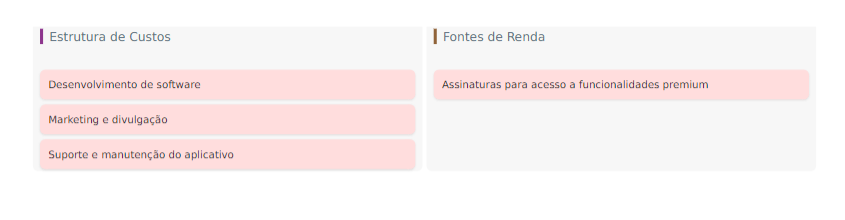
\includegraphics[width=0.9\textwidth]{Logos/canva2.png}
        \SourceOrNote{Sebrae (2024)}
        \end{figure}

 


\end{document}
